\section{GTFS-Madrid-Bench: Evaluation of Virtual Knowledge Graph Construction Engines}
\label{chapter5:sec-bench}


We have previously in Section \ref{chapter5:sec-param} identified several challenges for the development of a benchmark for virtual knowledge graph access that can be grouped into data, platform, output and mappings dimensions. In virtual KGC we have also to add the query dimension. The data and source challenges refer to having multiple data sources in an assortment of formats based on real-world data, and that can scale to large sizes. The challenges referred to queries point to SPARQL queries where different sources can be identified, where relations among sources (according to the specific data model) are exploited, and where necessary features of SPARQL are included to represent real-life use cases. Finally, the challenges related to the mapping dimensions is to include the relevant parameters that affect the generation of the virtual knowledge graph and give support to a set of declarative mapping languages.

To address these challenges, in this section, we describe a ``virtual knowledge graph access'' benchmark, GTFS-Madrid-Bench, that serves several purposes: (i) to evaluate and compare the performance of a mix of KGC engines that access several (homogeneous) sources in the same format, but where the mapping language used by each engine is specific to the data format considered; (ii) to evaluate virtual KGC engines over heterogeneous data sources; and (iii) to evaluate the strengths and weaknesses of both approaches. The general case of GTFS-Madrid-Bench is the comparison of the performance of KGC engines. The proposed GTFS-Madrid-Bench is composed of the following elements:

\begin{itemize}
    \item Several collections of sources in different formats (e.g. CSV, JSON, SQL, XML), which derive from the GTFS\footnote{The General Transit Feed Specification (GTFS) is a de-facto standard developed by Google for the description of public transport planning, routes and fares, among others. In recent years its popularity has increased thanks to its simplicity and the fact that it has not only been adopted by Google Maps, but also by other route planning systems such as Open Trip Planner or navitia.io.: \url{https://developers.google.com/transit/gtfs/}} feed from the metro system of the city of Madrid. These collections are scaled up so as to allow scalability testing.
    \item A set of mappings represented in the family of declarative languages that address different source formats (RML, R2RML, xR2RML, ontop OBDA mappings) that map the GTFS-based data sources into the Linked GTFS ontology\footnote{\url{https://github.com/OpenTransport/linked-gtfs}}.
    \item A set of 18 SPARQL queries of varied complexity.
    \item A set of well-established measurements~\citep{mora2013towards,lanti2015npd} that can be taken during the different phases of the KGC workflow~\citep{lanti2015npd,acosta2011anapsid}, such as query rewriting, query translation, query execution and query aggregation time.
\end{itemize}
GTFS-Madrid-Bench offers a fair environment for the comparison of different KGC engines, regardless of the mapping language that they have implemented, as long as the new mappings follow the same restrictions and specifications defined in the benchmark. Thus, newly released tools may be evaluated with the benchmark. Additionally, although we have generated our datasets from the GTFS feed of the city of Madrid metro system, any other city's GTFS feed may be used as data in the benchmark and the principles may be applicable to other types of datasets.

We provide a data generator to scale up the original data in terms of size, and distribute the datasets over different formats (e.g. JSON, XML, CSV, RDB). We demonstrate the use of GTFS-Madrid-Bench with four open source engines: Morph-RDB\footnote{\url{https://github.com/oeg-upm/morph-rdb}}, Ontop\footnote{\url{https://github.com/ontop/ontop}}, Ontario\footnote{\url{https://github.com/SDM-TIB/Ontario}} and Morph-xR2RML\footnote{\url{https://github.com/frmichel/morph-xr2rml}}. 

In summary, the main contributions of the work in this section are:
\begin{enumerate}
    \item C1: The proposal of a comprehensive and representative benchmark that includes a set of data sources, queries and mappings that allow evaluating and comparing multiple KGC engines for virtual knowledge graph access.
    \item C2: The extension of existing OBDA benchmark requirements to take into account (i) metrics that are commonly used in federated query processing benchmarks; and (ii) steps defined in new KGC engines~\citep{corcho2019towards}.
    \item C3: A data generation process where single and mixed data formats are scaled-up based on the features of the original data model, integrating state of the art data generator proposals for benchmark OBDA engines~\citep{lantivig}.
    \item C4: Evaluation of the proposed benchmark over five different engines, discussion of the obtained results and identification of the current limitations in the state of the art and future lines of work. 
\end{enumerate}


\subsection{Concepts and Definitions}

In this section, we introduce the main concepts and definitions that are later used to explain our work:

\paragraph{\textbf{Sources \& Dataset:}} we define a source as a tuple $\gamma=(\varphi,$ $\Sigma ,$ $f)$ where $\varphi$ is the data of any entity from our domain, $\Sigma$ is the model of the data, e.g. the columns of a CSV or the schema of a database table for SQL, and $f$ is a specific data format such as CSV, JSON, XML, or SQL, among others.% Remove this to go back to previous version
~ We define a dataset as a set of \textit{Sources}, i.e., $\mathcal{D}=\{\gamma_1,\gamma_2, ..., \gamma_n\}$. 

\textit{Example 1.} We define the following dataset $\mathcal{D}_{1}=\{(Rou\-tes,$ $\Sigma_1,$ $SQL),$ ($Stops,$ $\Sigma_2,$ $JSON)\}$ that involves the data of the metro routes (13 instances) and metro stops (1262 instances) in SQL and JSON formats, respectively. Both sources rely on different schemata $\Sigma_1$ and $\Sigma_2$, the first specifies the columns of a table and the second the keys of a JSON.

\paragraph{\textbf{Dataset Generator:}} we define a dataset generator as a function $\delta$ that takes as input a tuple ($\mathcal{D}$, $s$) where  $\mathcal{D}$ is a dataset and $s$ is a non-negative number that specifies a scale factor. The output of $\delta$ is a dataset $\mathcal{D'}$ containing enlarged versions, according to $s$, of the data ($\varphi$) within the sources of $\mathcal{D}$.

\textit{Example 2.} Assuming $\mathcal{D}_{1}$ from \textit{Example 1} and a scale factor $s$ of 2.5, a dataset generator may produce the following $\mathcal{D'}=\{(Rou\-tes{-}2.5,$ $\Sigma_1,$ $SQL),$ ($Stops{-}2.5,$ $\Sigma_2,$ $JSON)\}$. Notice that the schematas and the formats are the same, but the data of $Rou\-tes\-2.5$ and $Stops\-2.5$ has been scaled up from their versions in $\mathcal{D}_{1}$, containing 189 and 3536 instances respectively.

\paragraph{\textbf{Mapping:}} a mapping $m$ (already defined in Chapter \ref{chap:soa}) is a set of rules that specify the relationship between an ontology and the model of one or more sources. A mapping rule relates the elements within the schema of a source with elements from an ontology, including constants. In other words, a mapping rule $r$ contains the correspondences between an element $e$ within a schema of a source $\Sigma$ and an element $e_*$ of an ontology $\Sigma_*$. The ontology is known as unified view since it is the output of translating heterogeneous sources into the same model, i.e., the ontology.

\textit{Example 3.} Given the LinkedGTFS ontology and a CSV file with the columns ``id'' and ``route'', a mapping may state that each row generates a subject that includes the value of the column ``id', the predicate \textit{foaf:name} and its object with the corresponding value in the column ``route''.

\paragraph{\textbf{Experiment configuration:}} we define an experiment configuration $c$ as $(\mathcal{D}, q, M)$ where $\mathcal{D}$ is a dataset, $q$ is an SPARQL query and $M$ is a set of mappings.

\textit{Example 4.} We can specify the following experiment configuration $(\mathcal{D}_{1}, q1, \{shapes, trips\})$, where $\mathcal{D}_{1}$ is the data\-set specified in \textit{Example 1}, $q_1$ is the SPARQL query reported in Table~\ref{tab:queries}, 
and $M$ is the set of mappings $\{shapes, trips\}$  reported in Table~\ref{tab:mappings}.

\paragraph{\textbf{Processor:}} Given an experiment configuration $c$ and an ontology $\Sigma_*$, a processor represents a software component that encodes the function $\phi$ that takes as input a pair  $(c,\Sigma_*)$ and outputs a SPARQL result set $R$ ~\citep{w3c2013sparql}. 

Internally, the processor translates the SPARQL query $q$ into one or more queries expressed in different languages, depending on the formats within the dataset of $c$, using the mappings $M$. Then, the processor distributes and evaluates the queries and gathers the results. As a result, a unified result set is provided as output. This task is known as \textbf{Virtual Knowledge Graph Access}. We distinguish two kinds of processors: OBDA and OBDI. The former ones are able to handle only experiment configurations where all the data sources have the same data format. The latter ones are able to handle any experiment configuration, as discussed in Section \ref{sec:soa_engines}.



\subsection{Benchmark Proposal}

\begin{table}[t]
\caption{Virtual Knowledge Graph Access Benchmark Requirements}
\label{tab:req}
%\setlength{\tabcolsep}{1em}
\resizebox{0.8\textwidth}{!}{
\begin{tabular}{c|l}
\hline
\textbf{Variable} & \multicolumn{1}{c}{\textbf{Requirement}} \\ \hline
Ontology & \begin{tabular}[c]{@{}l@{}}The \textbf{ontology} should include classes with \\ data and  object properties \end{tabular} \\ \hline
Dataset & \begin{tabular}[c]{@{}l@{}}The \textbf{virtual instance} should maintain the constraints \\ defined in the original dataset\end{tabular} \\ \hline
Dataset & The \textbf{virtual instance} should be based on real world data \\ \hline
Dataset & \begin{tabular}[c]{@{}l@{}}The \textbf{virtual instance} should be distributed\\  in different data formats\end{tabular} \\ \hline
Mappings & \begin{tabular}[c]{@{}l@{}}The \textbf{mappings} should be able to indicate\\the format of the source\end{tabular} \\ \hline
Mappings & \begin{tabular}[c]{@{}l@{}}The \textbf{mappings} should be expressed\\using well known mapping languages\end{tabular} \\ \hline
Queries & The \textbf{query set} should be based on actual user queries \\ \hline
Queries & \begin{tabular}[c]{@{}l@{}}The \textbf{query set} should be complex enough with \\ relations among same but also different data sources\end{tabular} \\ \hline
Metrics & \begin{tabular}[c]{@{}l@{}}The \textbf{metrics} should provide relevant general information \\ but also specific measures for each defined phase\end{tabular} \\ \hline
\end{tabular}}

\end{table}


The GTFS-Madrid Benchmark consists of an ontology, an initial dataset of the metro system of Madrid following the GTFS model, a set of mappings in several specifications, a set of queries according to the ontology that cover relevant features of the SPARQL query language, a data generator based on a state of the art proposal~\citep{lantivig}, and a set of relevant metrics. In the following sections we describe in detail the resources of our virtual knowledge graph access benchmark. They are aligned with an extension of the requirements detailed in~\citep{lanti2015npd} (focused on benchmarks for OBDA) that we tailor to our context (Table \ref{tab:req}). All the resources described in this section are available online\footnote{\url{https://github.com/oeg-upm/gtfs-bench}}.

\subsubsection{The Linked GTFS Ontology} 
GTFS is a \textit{de-facto standard} developed by Google for the description of public transport schedules, routes, fares, etc. The specification defines the headers of 13 types of CSV files and a set of rules. Each file, as well as their headers, can be mandatory or optional and they have relations among them.

The Linked GTFS vocabulary\footnote{\url{https://github.com/OpenTransport/linked-gtfs}} can be seen as an ontology that represents the entities, properties and relationships described in the GTFS specification. The GTFS-Madrid-Bench mappings have been aligned to a subset of this vocabulary as the subway feed provides only the mandatory CSV files from the GTFS specification. Its conceptual model is shown in Figure \ref{fig:gtfsOntology} and a description of its classes is given in Table \ref{tab:GTFSClasses}. The ontology usually defines one class for each of the sources in the GTFS specification with the corresponding data and object properties, but there are some additions. The {\tt gtfs:Service} class represents information of the dates when a service (represented in GTFS in the files calendar and calendar\_dates) is available for one or more routes, the ontology also adds the {\tt gtfs:ServiceRule} class together with its two subclasses ({\tt gtfs:CalendarRule} and {\tt gtfs:CalendarDateRule})  to represent the service rules specified  in the calendar and calendar\_dates files. Finally, the class defined as \\{\tt gtfs:WheelchairBoardingStatus} and its three possible values (instances) have also been added to represent the corresponding field definitions in stops and trips. 

\begin{table}[t]
\caption{The LinkedGTFS Ontology: Classes and their Descriptions}
\label{tab:GTFSClasses}
%\setlength{\tabcolsep}{1em}
\resizebox{0.8\textwidth}{!}{
\begin{tabular}{c|l}
\hline
\textbf{Class} & \multicolumn{1}{c}{\textbf{Description}} \\ \hline
Agency & \begin{tabular}[c]{@{}l@{}} Agency that operates a certain transport mode
\end{tabular} \\ \hline
Stop & \begin{tabular}[c]{@{}l@{}} Physical location where a vehicle stops or leaves. 
\end{tabular} \\ 
 & \begin{tabular}[c]{@{}l@{}}  Multiple routes may use the same stop.
\end{tabular} \\ 
 & \begin{tabular}[c]{@{}l@{}} A stop may be wheelchair accessible.
\end{tabular} \\ \hline
Route & \begin{tabular}[c]{@{}l@{}} Collection of one or more trips.
\end{tabular} \\ 
 & \begin{tabular}[c]{@{}l@{}} Usually two trips in each direction.
\end{tabular} \\ \hline
Trips & \begin{tabular}[c]{@{}l@{}} A trip in a certain direction passes by stops.
\end{tabular} \\ 
 & \begin{tabular}[c]{@{}l@{}} A trip is associated with a shape.
\end{tabular} \\ \hline
StopTimes & \begin{tabular}[c]{@{}l@{}} An ordered sequence of stops. 
\end{tabular} \\
 & \begin{tabular}[c]{@{}l@{}} Includes their arrival and departure times.
\end{tabular} \\ \hline
Service & \begin{tabular}[c]{@{}l@{}} Set of dates when a service is available.
\end{tabular} \\ 
 & \begin{tabular}[c]{@{}l@{}} A Service  follows a rule that may have exceptions.
 \end{tabular} \\ \hline
 ServiceRule & \begin{tabular}[c]{@{}l@{}} May be a calendar rule or a calendar date rule.
\end{tabular} \\ \hline
CalendarRule & \begin{tabular}[c]{@{}l@{}} For a certain period, weekdays where active.
\end{tabular} \\ \hline
CalendarDateRule & \begin{tabular}[c]{@{}l@{}} Date to add or delete a service.
\end{tabular} \\ \hline
Shape & \begin{tabular}[c]{@{}l@{}} A polygon associated to a trip.
\end{tabular} \\ \hline
Frequency& \begin{tabular}[c]{@{}l@{}} Frequency of a trip.
\end{tabular} \\ \hline
 WheelchairBoardingStatus & \begin{tabular}[c]{@{}l@{}} Indicates whether wheelchair boarding is possible.
\end{tabular} \\ 
 & \begin{tabular}[c]{@{}l@{}} Available for a trip or a stop.
\end{tabular} \\ \hline
\end{tabular}}
\end{table}

In general, all the ontology classes have been populated except for {\tt gtfs:FareClass} and {\tt gtfs:FareRule} because the Madrid GTFS data does not contain information on these two entities. The {\tt gtfs:RouteType} class is not considered because the data covers only the Metro system.


\begin{figure}
    \centering
    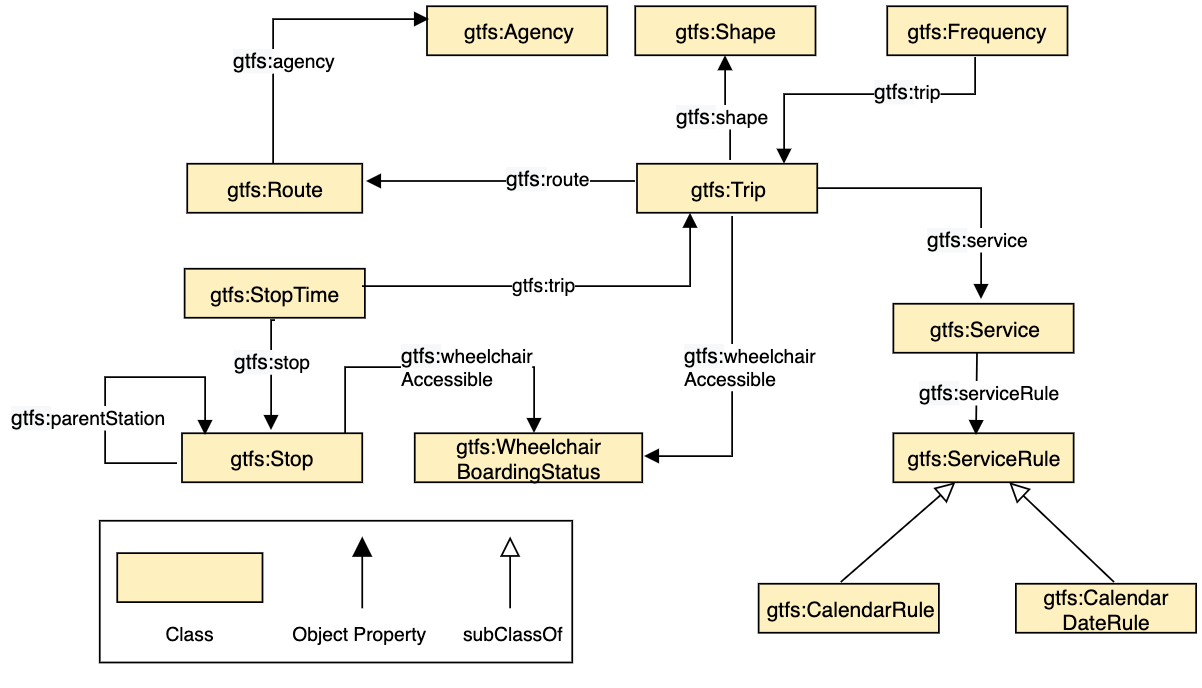
\includegraphics[width=1\linewidth]{figures/GTFSontology.png}
    \caption[The LinkedGTFS Ontology]{\textbf{LinkedGTFS Ontology.} Subset of the LinkedGTFS ontology used in the GTFS-Madrid-Bench for virtual knowledge graph access. There are eleven object property relations among the classes, and two subClassOf relations.}
    \label{fig:gtfsOntology}
\end{figure}

\subsubsection{Dataset Generation}

Dataset generation for a virtual knowledge graph access benchmark should be focused on the two main variables that allow testing the capabilities of the engines: (i) data size, and (ii) formats in which data can be expressed. In the context of data generation for OBDA, VIG~\citep{lantivig} proposes the use of R2RML mappings for an efficient scale up of the size of an instance of an RDB dataset. In this case, only one data format (SQL) is involved in the process. 

We use GTFS as the original data source for several reasons: First, GTFS has been the \textit{de-facto} standard for publishing transport data on the web, it also comes with a clear specification, making it easy to understand. Second, the GTFS model comprises several entities that are related through a variety of relationships. In addition it includes different data types such as strings, integers, and booleans. Finally, many cities have adopted the GTFS data model and have published their GTFS data online.

The GTFS-Madrid-Bench proposes an extended workflow using VIG as the Dataset Generator engine for the generation of the datasets taking into account multiple data formats (see an example in Figure \ref{fig:generation}). We describe the detailed steps of the proposed data generation workflow together with examples:

\begin{enumerate}[label=\textbf{\arabic*})]
    \item \textbf{Data preparation.} The original data source, GTFS, is in CSV format. VIG requires an instance of an RDB and an R2RML mapping for scaling up the data source. We use Morph-CSV~\citep{chaves2020enhancing} (describe in Section \ref{chap6_morphgcsv}), which takes as inputs a set of spreadsheets in the form of CSV files, their corresponding annotations using CSVW~\citep{tennison2015model} and an RML mapping~\citep{dimou2014rml}. It automatically produces the corresponding schema of an RDB (identifying typical constraints such as datatypes, PK/FK, indexes and NULLs) and an R2RML mapping document, which are the inputs for VIG. 
    
    For the Madrid-GTFS-Bench, we use as input an open data dataset GTFS$_{mad}^{CSV}$ = (GTFS$_{mad}$, GTFS, CSV). GTFS$_{mad}$ is the set of data sources of the subway network of Madrid that have been provided by its transport authority according to the GTFS schema as described in its specification\footnote{\url{https://developers.google.com/transit/gtfs/}}. This dataset is composed of a set of CSV files containing data of Agency, Route, Shape, Frequency, Trip, StopTime, Stop, Calendar and CalendarRule. This input is fixed during all of the data generation process, which means that the generated datasets are defined by the same schema and all of the generated data is obtained from this initial dataset. We create the corresponding RML mapping rules and CSVW metadata annotations and, using the Morph-CSV engine, we generate the corresponding RDB instance GTFS-SQL-1=(GTFS$_{mad}^{SQL}$,1) dataset and the R2RML mapping rules.
    
    \item \textbf{Data creation.} VIG~\citep{lantivig} takes into account the ontology and the set of R2RML mappings to generate each dataset. This engine also receives as input a scale value $s$ that indicates that the size of each table of the database increases $s$ times. The output of VIG is a set of CSV files, one file for each table of the RDB. In this step the dataset GTFS-CSV-s=(GTFS$_{mad}^{CSV}$,s) is generated, where $s$ is the selected scale value.
    
    \item \textbf{Data distribution.} Finally, each dataset generated using VIG is distributed in several formats. We use open source tools to perform this step such as csv2json, from Python CSVKit\footnote{\url{https://csvkit.readthedocs.io/en/1.0.3/scripts/csvjson.html}} and di-csv2xml\footnote{\url{https://github.com/blue-yonder/di-csv2xml}}, depending on the data formats (JSON and XML). We divide the distribution into two categories in order to cover both OBDA and OBDI approaches: 
    
    In the first category, focused on providing support to OBDA techniques, the sources of each dataset are transformed into a single format (e.g., CSV files are transformed into JSON files). The datasets are transformed to the corresponding ones in JSON, XML, SQL and MongoDB obtaining the following datasets: GTFS-F-s$=$(GTFS$_{mad}^{F}$,s) where $s$ is the scale value and F $\in$ $\{$JSON, XML, SQL, MongoDB$\}$. 
    
    In the second category, focused on virtual KGC approaches, the sources of each dataset have to be transformed from the CSV files into multiple formats (e.g. CALENDAR is a JSON document, AGENCY is a XML file, etc.). To distribute the files and based on the GTFS model, the user may select the sources associated to each format and then the benchmark generates the dataset and the corresponding set of mapping rules. For example, a parameter that can be studied is the join selectivity. The value of this parameter between shapes and trips is different than between routes and agencies, and depending on the format of each source, the total query execution time of a processor may be impacted. Other parameters such as the number of joins among sources in same/different formats and the impact of the data size in different sources can also be studied.
   
\end{enumerate}
 
\begin{figure}
    \centering
    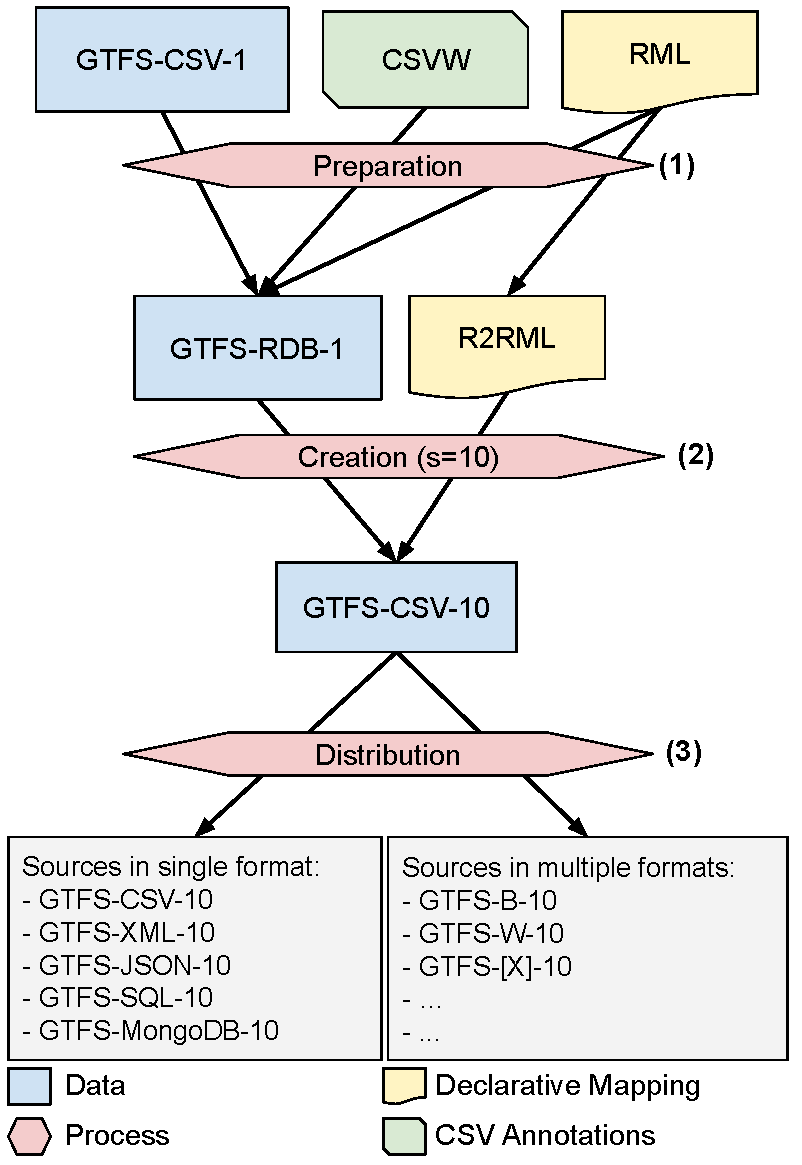
\includegraphics{figures/gprocess.pdf}
    \caption[Generation workflow for scale value 10]{\textbf{GTFS-Madrid-Bench Generation Workflow with scale value 10}. From the original 10 CSV files of Madrid Metro GTFS we use (i) Morph-CSV to generate the corresponding RDB instance and an R2RML mapping that are the required inputs for (ii) scaling up the data using VIG and (iii) distributing the generated CSV dataset to the different formats.}
    \label{fig:generation}
\end{figure}

We want to be able to compare the results obtained by processors with the results obtained by the materialized graph in RDF. For this purpose, we take the output of VIG (e.g., GTFS-CSV-5, GTFS-CSV-10) and we run a materialized KGC process using the SDM-RDFizer~\citep{iglesias2020sdm} (described in Section \ref{chap7_rdfizer}) engine, which generates the KG in RDF using RML mapping rules. We select this tool because it passed all the RML Test Cases~\citep{heyvaert2019conformance} for CSV files\footnote{\url{http://rml.io/implementation-report/}}, hence we assume that the generation is correct, and that it provides a set of techniques to optimize the generation of RDF at scale. 

\begin{table}[t]
\centering
\caption[Mapping Features for transforming LinkedGTFS to GTFS]{\textbf{Mapping Features for transforming LinkedGTFS to GTFS.} Each TriplesMap of the GTFS mapping file and its corresponding features: the related source, number of Classes, PredicateObjectMaps, Predicates, Objects and RefObjectMaps (joins). }
\label{tab:mappings}
\resizebox{1\textwidth}{!}{%
\begin{tabular}{l|l|l|c|c|c|c}
\hline
\multicolumn{1}{c|}{\textbf{TriplesMap}} & \multicolumn{1}{c|} {\textbf{Source}} & {\textbf{Classes}} & \textbf{\#PredicateObjectMap} & \textbf{\#Predicates} & \textbf{\#Objects} & \textbf{\#RefObjectMap} \\ \hline
shapes          &  shapes              & gtfs:Shape                               & 4                     & 4            & 4         & 0      \\ \hline
trips           &  trips              & gtfs:Trip                               & 8                     & 8            & 5         & 4      \\ \hline
calendar\_rules         & calendar              & gtfs:CalendarRule                               & 9                     & 9            & 9         & 0      \\ \hline
calendar\_date\_rules   &  calendar\_dates            & gtfs:CalendarDateRule                               & 2                     & 2            & 2         & 0      \\ \hline
stops              &    stops         & gtfs:Stop                               & 12                    & 12           & 11        & 1      \\ \hline
stoptimes         & stop\_times           & gtfs:StopTime                               & 9                     & 9           & 7         & 2      \\ \hline
routes               &  routes         & gtfs:Route                               & 8                     & 8            & 7         & 1      \\ \hline
agency                & agency          & gtfs:Agency                               & 6                     & 6            & 6         & 0      \\ \hline
frequencies       &  frequencies              & gtfs:Frequency                               & 5                     & 5            & 4         & 1      \\ \hline
feed      &  feed\_info               & gtfs:Feed                               & 6                     & 6            & 6         & 0      \\ \hline
service1 &   calendar           & gtfs:Service                               & 1                     & 1            & 0         & 1      \\ \hline
service2 & calendar\_dates       & gtfs:Service                               & 1                     & 1            & 0         & 1      \\ \hline
\textbf{Total}      &  \multicolumn{1}{c|}{10}    & \multicolumn{1}{c|}{11}                           & 71                     & 71            & 60         & 11      \\ \hline
\end{tabular}%
}

\end{table}

\subsubsection{Mappings} 
Mappings play one of the most important roles in the benchmark since they are the main element used for the query translation process. In the state of the art there are multiple engines and tools that use different mapping languages. We select a set of the most relevant declarative mapping languages in the state of the art and we generate the corresponding mapping rules. In more detail, the GTFS-Madrid-Bench provides:
\begin{itemize}
    \item One R2RML mapping document for accessing SQL datasets.
    \item One xR2RML mapping document for accessing MongoDB datasets.
    \item Seven RML mapping documents\footnote{Provided in RML and YARRRML serializations} for accessing CSV, JSON, XML, SQL, MongoDB, Best and Worst datasets.
    \item One CSVW metadata file to provide annotations for the CSV datasets.
\end{itemize}
Conceptually, all the mappings represent the same relations among the concepts of the ontology and the concepts of the GTFS model, but each one has been developed according to a specification that handles the characteristics of each data format. The mappings are composed by a set of rules representing the relation of one element in the ontology with the corresponding schema element from a source. An overview of the rules within the mappings developed for this benchmark is shown in Table \ref{tab:mappings}. The rules of the mappings are very relevant since they contain many parameters that impact on the performance of the virtual knowledge graph access engines~\citep{chaves2019what}. 

More in detail, each source of the GTFS feed has one associated TriplesMap with a rule to associate the generated entities to the class defined in the ontology, and a set of rules for the object and data properties. Additionally, there is a (virtual) entity, Service, in the data model with no corresponding source, what implies the definition of a set of mapping rules to generate the instances of the corresponding class (\texttt{gtfs:Service}). Following the GTFS specification, the identifier of Service can be found either in calendar or calendar\_dates sources. This means that to be aligned with standard declarative mapping specifications (e.g. RML and R2RML only allow one source per TriplesMap), the mapping document needs to define two TriplesMap, one for calendar (service1) and another for calendar\_dates (service2). This also implies that the trips TriplesMap has one predicate (\texttt{gtfs:service}) with two associated refObjectMaps, where the parentTriplesMap are service1 and service2; this allows generating all \texttt{gtfs:Service} defined in the original data source. Because the instances of \texttt{gtfs:WheelchairBoardingStatus} class are only objects in \texttt{gtfs:Trips} and \texttt{gtfs:Stops} triples, they are generated using the template property in trips and stops TriplesMap. In summary, the mapping contains rules to generate instances of 12 classes, 71 PredicateObjectMaps and Predicates, 60 Objects and 11 RefObjectMaps, covering the main features defined in state-of-the-art mapping specifications for KGC. All of the GTFS mappings are detailed in Appendix \ref{sec:appendix2} using the YARRRML~\citep{Heyvaert2018Declarative} serialisation.

% Queries
\subsubsection{Queries}
Table \ref{tab:queries} presents all the variables considered for the 18 queries in our benchmark. We have developed queries that are based on the Linked GTFS ontology, and are aligned with user stories in Madrid's transport domain, together with different combinations of values for the variables. It should be mentioned that the queries cover all of the data sources that were generated by the Madrid's transport authority as GTFS data from the metro system. These include agencies, routes, stops, trips, frequencies, shapes, calendar, and calendar dates. Although in the benchmark we have defined mappings to translate queries into the underlying query language of the source, these are independent from the queries (we have used these mappings to generate the materialized knowledge graph in the data generation step).

\begin{sidewaystable*}[p]
\centering
\caption{Description of the GTFS-Madrid Benchmark Queries}
\label{tab:queries}
\resizebox{1\textwidth}{!}{%
\begin{tabular}{c|l|c|c|c|c|c|c|c|c|c}
\hline
%Query & Description & \#Triple  & \#Sources & OPTIONAL & Aggregation & Other & FILTER & FILTER & Star-shaped groups  \\ 
Query & Description & \#Triple  & \#Sources & OPTIONAL & Aggregation & Other & \multicolumn{2}{ |c| }{FILTER} & \multicolumn{2}{ |c }{\#Star-shaped groups} \\   
 &  & Patterns  &  & &  & features  & equal to & relational  &  w/o constants & w/constants \\ \hline
q1 & All shapes & 4 & 1 &  &  &  &  &  & 1 & 0 \\ \hline
q2 & All stops where the latitude is larger than a & 5 & 1 & \checkmark &  &  &  & \checkmark & 0 & 1 \\ 
&  specific value &  &  &  &  &  &   &   &  & \\ \hline
q3 & Accessibility information of all stations & 5 & 1 & \checkmark &  &  & \checkmark &  & 0  & 1 \\ \hline
q4 & All agencies and their routes & 9 & 2 & \checkmark &  &  &  &  & 2 & 0 \\ \hline
q5 & Services that have been added after a specific date& 5 & 2 &  &  &  &  & \checkmark & 1 & 1 \\ \hline
%&  specific date  &  &  &  &  &  &   &   &  & \\ \hline
q6 & Number of routes covered by a specific agency & 3 & 2 &  & \checkmark &  & \checkmark &  &  0  & 2 \\ \hline
q7 &  All wheelchair-accessible stops in a specific route   & 15 & 4 & \checkmark &  & DISTINCT & \checkmark &  & 1 & 3 \\ \hline
q8 & Routes and their related trips, services, stops and stop times & 14 & 5 & \checkmark &  &  &  &  & 5 & 0 \\ \hline
q9 &  Trips and associated shapes where latitude  & 7 & 2 & \checkmark &  &  &  & \checkmark & 1 & 1 \\ 
 &  is larger than a specific value &  & &   &  &  &   &  &   &   \\ \hline
q10 &  Number of trips that have a duration   & 4 & 2 &  & \checkmark & DISTINCT &  & \checkmark & 1 & 1 \\ 
 &  over a number of minutes &  &  &  &  &  &   &   &  & \\ \hline
q11 & Trips that are available on a certain date  & 12 & 3 &   &  & NOT EXISTS &  & \checkmark & 3 & 2 \\ \hline
 %&  &  &  &   &  &  &  &  &  & \\ \hline
q12 & Number of stops that are wheelchair-accessible  & 10 & 4 &   & \checkmark & GROUP BY &  &  & 3 & 1 \\ 
 & grouped by route  &  &  &   &  &  &  &  &  & \\ \hline 
q13 & The accesses of all stations & 6 & 1 &  \checkmark &  &  &  &  & 0 & 1 \\ \hline
q14 & All stops times and their related routes and stops ordered by  & 8 & 3  & \checkmark &  & ORDER BY &  &  & 3 & 0 \\ 
  & their sequence, in a specific direction and service  &  &   & &  &  &  &  & & \\ \hline
q15 & For all properties, triples that contain  & 3 & 1 &    &  &  & \checkmark &  & 0 & 1 \\ 
 &  a specific  word in the object placeholder  &  &  &    &  &  &  &  & & \\ \hline
q16 & For all routes, all calendar changes in  & 8 & 3 &    &  &  &  & \checkmark & 2 & 1 \\ 
 &  a specific month &  &  &    &  &  &  &  & & \\ \hline
q17 & Trips with their start and end time  & 9 & 3 &   &  &  &  &  & 3 & 0 \\  
 & of the frequencies and associated routes    &  & &   &  &  &  &  & & \\  \hline
q18 & All routes that have trips on Sunday  & 8 & 5 &   &  & UNION &  &  & 4 & 1 \\ \hline 
\end{tabular}%
}
\end{sidewaystable*}


\subsubsection{Metrics}
In this section we define the metrics that are used to evaluate the performance of Virtual Knowledge Graph access engines. The metrics consider the workflow followed by Virtual Knowledge Graph systems, and for each of the steps identified in the workflow we introduce a set of metrics to be measured and reported.
\begin{table}[t]
\caption[Comparison between Benchmark Metrics and Dimensions]{\textbf{Comparison between Benchmark Metrics and Dimensions.} Relation between each relevant metric for the Madrid-GTFS-Bench and the dimensions that can impact over that metric. In the Dimension column, Q means query, M mappings and D data.}
\label{tab:dimsensions}
\begin{tabular}{l|c|c}
\hline
\multicolumn{1}{c|}{\textbf{Metric}} & \textbf{Type or Phase} & \textbf{Dimension}  \\ \hline
\multicolumn{3}{c}{General Metrics}                                                 \\ \hline
Total execution time                & General                & D, Q, M \\ \hline
\# answers                            & General                & D, Q, M \\ \hline
Initial delay                         & General                & D, Q, M \\ \hline
Dief@k                                & C. Behaviour           & D, Q, M \\ \hline
Dief@t                                & C. Behaviour           & D, Q, M \\ \hline
\multicolumn{3}{c}{Specific Metrics (Phases)}                                       \\ \hline
Loading time                          & Starting        & Q, M      \\ \hline
Mapping translation time              & Starting         & M              \\ \hline
\# requests                           & Distribution      & Q              \\ \hline
Source selection time                 & Distribution      & Q, M     \\ \hline
Query generation time                 & Distribution      & Q               \\ \hline
Query rewriting time                  & Rewriting     & Q                \\ \hline
Query translation time                & Translation    & Q, M       \\ \hline
Query execution time                  & Execution     & Q, D          \\ \hline
Query aggregation time                & Finishing         & D                 \\ \hline
\end{tabular}
\end{table}

The workflow extends the OBDA phases identified by~\citep{mora2013towards}, and~\citep{lanti2015npd}. In addition, it includes some of the steps that are defined by proposals that federate queries~\citep{schwarte2011fedx}. General metrics to be captured are \textbf{overall execution time}, \textbf{completeness of answers} and \textbf{initial delay}. Other metrics may be considered when the engine generates answers following a continuous behavior~\citep{sharaf2008algorithms}, such as \textbf{dief@k} or \textbf{dief@t} proposed in \citep{acosta2017diefficiency}. Additionally, for each phase of a workflow, a virtual knowledge graph construction engine may capture specific metrics that allow the identification of bottlenecks in the implementations. This relevant set of metrics for each phase are: (i) \textbf{loading time} during the starting phase when the ontology, mappings and query are loaded; (ii) \textbf{total number of requests} and \textbf{source selection time} during the source selection phase (the engine identifies the sources that can be used to answer the query); (iii) \textbf{query generation time} when the set of sub-queries to be evaluated over each data source is created, and the query plan is generated; (iv) \textbf{mapping translation time} when the engine requires to translate a provided mapping into another one in in a different language, maintaining a set of properties between them~\citep{corcho2019towards}; (v) \textbf{query rewriting time} when the generated sub-queries are rewritten to other queries, taking into account potential inferences from the ontology and information in the mapping~\citep{mora2014kyrie2}; (vi) \textbf{query translation time} when the engine, taking the mapping into account, translates each sub-query to another one in the query language supported by the underlying data sources such as SPARQL-to-SQL~\citep{chebotko2009semantics}; (vii) \textbf{query execution time} when the translated queries are evaluated against the underlying data sources and the results are translated to RDF or as SPARQL bindings using the rules provided in the mappings; and (viii) \textbf{query aggregation time} when the results obtained for each sub-query are aggregated, including the removal of duplicates and the linking of resources. Variables that have an impact on the metrics have been grouped into three dimensions: Query, Data, and Mappings. The relation between each  metric considered  and the dimensions that can impact over that metric is  shown in Table \ref{tab:dimsensions}.

\noindent\paragraph{\textbf{Query.}} The Query dimension variables refer to the structure of the queries, e.g. \#triple patterns, \#sources, and  \#star-shaped groups. A  Star-shaped group is a group of triple patterns that are ``joined" over the same subject or object variable~\citep{vidal2010efficient}. The most common case in real-world scenarios are subject star-shaped groups that represent properties that describe one source. The benchmark considers an increasing number of triple patterns, from 3 to 15, also the number of sources vary from 1 to 5. In particular we have several queries on 1 source with a varying number of triple patterns, and queries that have a large number of triple patterns combined with 4 and 5 sources. With respect to these two variables, our aim is to balance real-life use cases where several properties in the specification need to be combined and retrieved, and query complexity (worst case scenario is the ``Worst Dataset'' when the five sources are represented in the five available formats and the number of joins among sources is maximized).Furthermore, a large number of sources or triple patterns  combined with a large number of non-instantiated star-shaped groups should impact overall execution time and also specifically impact query generation, query rewriting, query translation, and query execution times. 

In general, queries in GTFS-Bench-Madrid combine those that contain single star-shaped groups ($q1$,$q2$, $q3$, $q15$) with those that contain chains of star-shaped groups, that is, where the object of a pattern in a group is the subject in the next group (with joins across different sources): $q4$, $q5$, $q6$, $q7$, $q9$, $q10$, $q11$, $q12$, $q16$, $q17$, $q18$. According to the ontology structure shown in Figure \ref{fig:gtfsOntology}, \texttt{gtfs:StopTime} relates to stops and trips and may lead to hybrid shapes such as $q8$ and $q14$. There is also the case of query $q13$, which refers one source and contains a self-join that relates an access to a station to its ``parent'' station.

Besides, as mentioned in~\citep{montoya2012benchmarking}, query plans generated by query evaluation systems during the subquery generation phase may be affected by the structural properties of a query. If the sources in the dataset are all represented in the same format, then query plans will be generated by the underlying engine (either an RDB engine or a NoSQL engine), and execution time will be affected by the number of joins within star-shaped groups and among these groups. When the sources of the dataset are not in the same format, the engine has to create the query plan. The performance will be affected by the plan proposed by the engine. Different combinations of these variables are considered in GTFS-Madrid-Bench queries: on the one hand we have a large number of triple patterns, sources and star-shaped groups in $q7$ and $q8$, and on the other hand queries like $q18$ combine a large number of sources and star-shaped groups with a medium-sized query (8 triple patterns).

Complexity of SPARQL queries is presented in~\citep{perez2009semantics}, considering the SPARQL fragment with only AND and FILTER operators. Complexity is linear on the product of the dataset size and the size of the query (\# triple patterns), and evaluation is NP-complete for queries constructed with AND, FILTER and UNION operators. Several queries in GTFS-Madrid-Bench have FILTER clauses and specifically, $q18$ contains a UNION of two triple patterns.

The evaluation problem becomes harder when the OPTIONAL operator is added~\citep{perez2009semantics}. Additionally, the work described in~\citep{xiao2018efficient} presents optimization techniques applied in an OBDA setting specifically for queries that have to deal with OPTIONAL triple patterns, claiming that the underlying database systems do not optimize adequately these class of queries. Similar problems may be expected for querying CSV, XML and JSON data sources. We have designed eight queries that use OPTIONAL graph patterns (according to the corresponding non-mandatory attributes in the specification). 

Constants in triple patterns together with FILTER with equality operators increase the selectivity of queries and are likely to reduce the cost of evaluating the query. According to~\citep{montoya2012benchmarking}, instantiated triple patterns have an important impact on the potential number of join intermediate results that may be generated throughout query execution. However, using a FILTER relational operator specially in the case of open ranges, e.g. a FILTER with a $>$ operator, may generate a large number of answers. We have considered several combinations of number of star-shaped groups with and without constants, $q8$ has no constants whereas in $q4$ both star-shaped groups in the query have bindings. An example of an intermediate case occurs in $q12$ with 1 out of 4 instantiated star-shaped groups. 

Three queries contain the aggregated COUNT function, and one of these queries contains additionally the GROUP BY modifier. Other queries use language features like DISTINCT and ORDER, what will impact on the query execution time metric because all of them require an ordering of the tuples/entries of the underlying sources. We cover the impact of these variables in $q7$ and $q10$ with DISTINCT, and $q12$ and $q14$ with GROUP BY and ORDER BY respectively. Finally, having unbounded predicates in a query ($q15$) increases its complexity because the search space during query evaluation may be large. 

The work in~\citep{angles2016negation} studies the impact of negation in the computational complexity of SPARQL queries, it distinguishes four types of negation: negation of filter constraints, negation as failure, negation by MINUS and negation by NOT EXISTS.  The use of NOT EXISTS introduces similar issues to sub-query evaluation because of the  presence of correlated variables and the use of a nested iteration method to evaluate queries that contain this type of negation. Hence $q11$ contains negation with NOT EXISTS.


\noindent\paragraph{\textbf{Mappings.}}
Features of mappings are relevant because they may impact  the performance of the engines. Previous work by~\citep{chaves2019what} evaluates different mapping variables that impact in the construction of a knowledge graph. Similarly, we consider that the following mapping variables influence overall query execution time and specifically query translation and query rewriting times. Regarding structure, we have considered the variables \#Classes, \#PredicateObjectMaps, \#Predicates, \#Objects, and \#RefObjectMap that are presented in Table \ref{tab:mappings}. Another variable is relation type, the mappings of the Madrid-GTFS-Bench include 1-1, 1-N, N-1 and N-M relation types. In general mappings for sources that represent N-M relationships (e.g. stop\_times) are more complex and thus time consuming for query execution. Additionally, the variable \texttt{rr:termtype} of the \texttt{rr:objectMap} may also have an effect because the cost of generating a constant, a reference or a template is not the same.

\noindent\paragraph{\textbf{Dataset.}}
Variables in this dimension include dataset size and the formats of its sources. As already mentioned, datasets with different scale factors are generated in GTFS-Madrid-Bench. Size has an impact on the overall execution time, on the initial delay, and specifically on query execution time because of the larger number of intermediate results. It also influences query aggregation time because in the benchmark, queries against larger datasets generate a larger number of answers.

The format variable may take a single value for datasets in only one format (RDB, CSV, XML, MongoDB, JSON) or multiple formats (Best, Worst and Random). This variable has an impact on the overall execution time, specifically on the query translation and query execution times, as well as on the number of answers because  different formats have different access methods and different underlying query languages.

The work in~\citep{montoya2012benchmarking} presents partitioning and data distribution in this dimension. In GTFS-Bench-Madrid there are fixed values for these variables: the partitioning is vertical and datasets and databases are loaded in local machines.


\subsection{Experimental Evaluation}
In this section we describe the evaluation performed using our benchmark. We first describe the selected virtual KGC engines involved in the evaluation, we describe the evaluation methodology and infrastructure, based on the use of docker images to ensure the reproducibility of the experiments, and finally, we provide the obtained results. All the resources used in this evaluation, such as queries, data, mappings, running scripts, results and docker images for engines and databases are publicly available online\footnote{\url{https://github.com/oeg-upm/gtfs-bench}}.

\subsubsection{Tools}

We selected the most relevant open source virtual KGC engines in the state of the art (described in Section \ref{sec:soa_engines}): Ontario, Ontop, Morph-RDB and Morph-xR2RML. We also intended to include other engines such as Squerall~\citep{mami2019querying} or Polyweb~\citep{khan2019one}. In both cases, either the code is not available as open source or it was not feasible to run the engine due to the lack of documentation. Issues have been reported in their corresponding repositories, with the intention of alerting the authors and maintainers about the current limitations.

\subsubsection{Setup}
In this section we describe how we use our benchmark to evaluate several processors/engines. We have setup several experiment configurations for evaluating the selected processors. As an example, the experiment configurations for query $q4$ can be seen in Table \ref{tab:ExperimentalEnvironment}. These experiment configurations have a fixed set of mappings with routes and agencies. The processor used to evaluate this query depends on the dataset, for example, Ontario in the case of the JSON dataset or Morph-RDB, Ontario and Ontop for SQL.
\begin{figure}[t]
    \centering
    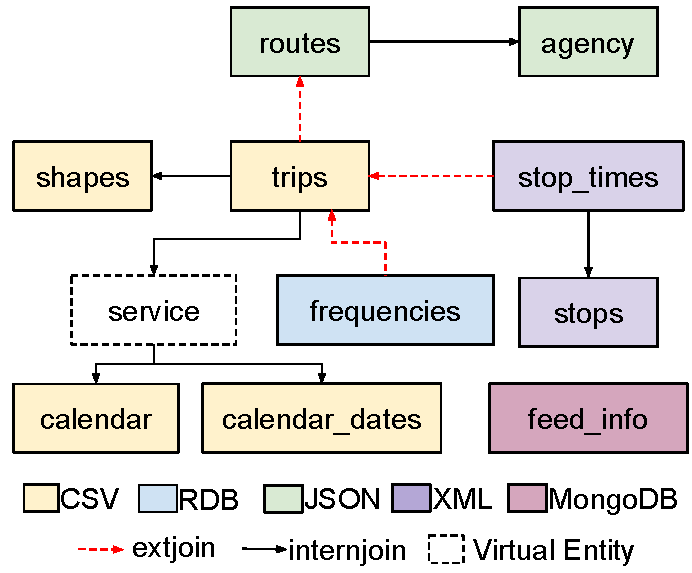
\includegraphics[width=0.75\linewidth]{figures/best-dist.pdf}
    \caption{\textbf{Example of MINEXTJ dataset}. GTFS$_{mad}^{minextj}$ dataset distributes the formats over the data sources ensuring that at least there is one source per each format and the joins among different formats are minimised. \textit{extjoin} means that there is a relation between sources in different formats and \textit{internjoin} means that the joins are between sources in the same format.}
    \label{fig:best}
\end{figure}
\begin{figure}[t]
    \centering
    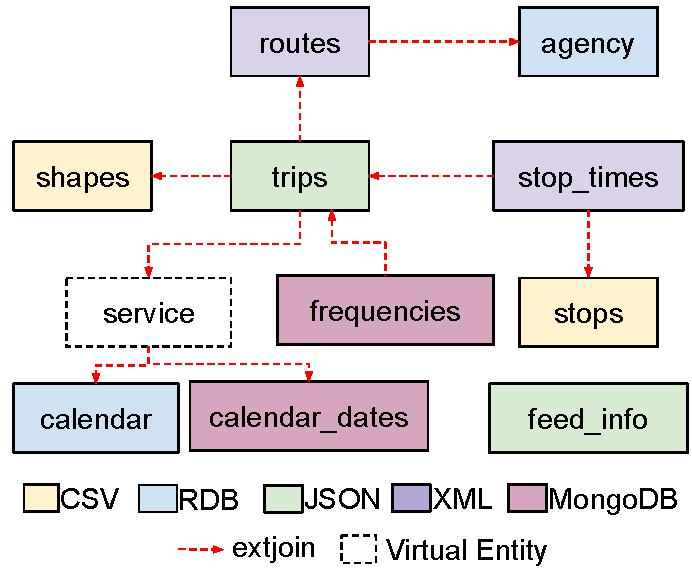
\includegraphics[width=0.75\linewidth]{figures/worst-dist.pdf}
    \caption{\textbf{Example of MAXEXTJ dataset}. GTFS$_{mad}^{maxextj}$ dataset distributes the formats over the data sources ensuring that at least there is one source per each format and the joins among different formats are maximised. \textit{extjoin} means that there is a relation between sources in different formats.}
    \label{fig:worst}
\end{figure}


\begin{table}[t]
\centering
\caption[Experiment configuration example set]{\textbf{Experiment configuration example set.} List of experimental configurations and processors for q4. $D$ is a dataset where $s$ is the scaling factor (i.e., 1, 5, 10, 50, 100, 500), $M$ is the set of mappings, $q$ is the SPARQL query, $\phi$ is a processor. $q$ is a SPARQL query defined in the Appendix Section.}
\label{tab:ExperimentalEnvironment}
\resizebox{0.85\textwidth}{!}{%
\begin{tabular}{c|c|c|c}
\hline
\textbf{Query $q$} & \textbf{Dataset $D$} & \textbf{TriplesMap $M$} & \textbf{Processor $\phi$} \\ \hline
\multirow{10}{*}{q4} & \multirow{2}{*}{GTFS$_{mad}^{csv}$-s} & \{routes,agency\}$_{R2RML}$ & Morph-RDB \\ \cline{3-4} 
 &  & \{routes,agency\}$_{RML}$ & Ontario \\ \cline{2-4} 
 & \multirow{3}{*}{GTFS$_{mad}^{sql}$-s} & \{routes,agency\}$_{R2RML}$ & Morph-RDB \\ \cline{3-4} 
 &  & \{routes,agency\}$_{RML}$ & Ontario \\ \cline{3-4} 
 &  & \{routes,agency\}$_{OBDA}$ & Ontop \\ \cline{2-4} 
 & GTFS$_{mad}^{mongodb}$-s & \{routes,agency\}$_{xR2RML}$ & Morph-xR2RML \\ \cline{2-4} 
 & GTFS$_{mad}^{xml}$-s & \{routes,agency\}$_{RML}$ & Ontario \\ \cline{2-4} 
 & GTFS$_{mad}^{json}$-s & \{routes,agency\}$_{RML}$ & Ontario \\ \cline{2-4} 
 & GTFS$_{mad}^{minextj}$-s & \{routes,agency\}$_{RML}$ & Ontario \\ \cline{2-4} 
 & GTFS$_{mad}^{maxextj}$-s & \{routes,agency\}$_{RML}$ & Ontario \\ \hline
\end{tabular}%
}
\end{table}


All the experiment configurations are loaded into a machine with the following characteristics: 2GHz CPU with 15 cores, 32 RAM, 200 GB HDD with Ubuntu 18.04 as its operating system. The machine contains a docker image for each of the processors: Morph-RDB v3.12.5, Ontop v3.0.0, Ontario v.0.3, Morph-xR2RML-1.1-RC2. All the engines are configured with the recommended settings provided in the corresponding online repository. 

In terms of data size, we decide to evaluate the engines over the scale values (5, 10, 50, 100 and 500). After some preliminary tests, we observed that these values provide a good overview of the current state of the engines in terms of query evaluation performance. For each SQL dataset size, we create two docker images where the data is loaded, one as an instance of the MySQL Database Server v5.5 and another as an instance of the MySQL Community Server v8.0. Similarly, for each MongoDB dataset size, we create a docker image of an instance of the MongoDB Community Server v3.4 with the dataset is loaded. The rest of the datasets, which correspond to raw data (CSV, XML and JSON), are loaded into the machine and are accessible to all the processors. 

To test OBDI engines and to demonstrate the capabilities of the benchmark resources covering multiple scenarios, we chose to analyze the impact of the number of joins among different formats. The main reason to test this paremeters is because Ontario is focused on improving the performance of these kind of queries. The dataset were created taking into account the selected formats (JSON, CSV, XML, SQL and MongoDB) and varying the number of relations (joins) among different formats. More specifically, the dataset distributions are the following:

\begin{itemize}
    \item MINEXTJ dataset: The number of joins among sources in different formats is minimized but ensuring that all of the formats are covered. The aim of this configuration is to study the behavior of the engines when they have to deal with different data sources but where most of the joins are done between sources in the same format. Hence they may delegate their treatment to the underlying data source manager (e.g. MySQL in RDB) and apply common optimization techniques in query translation approaches~\citep{priyatna2014formalisation}. To meet this requirement and, having 5 possible formats for the data sources, the proposed groups for this dataset are: trips, shapes, calendar and calendar\_dates sources in one group, routes and agency in another, frequencies in the third group, stop and stop\_times in the fourth one and feed\_info in the last one. This composition generates the GTFS$_{mad}^{MIN-EXTJ}$ dataset. We show the used dataset in the evaluation in Figure \ref{fig:best}. 
   
    \item MAXEXTJ Dataset: The number of joins among sour\-ces in different formats is maximized and the five formats are covered. In this distribution, all the possible joins are among sources in different formats. This means that the OBDI engine may be enforced to perform the joins after the execution of the translated queries over the original data sources. In the same manner as the minimized dataset, the groups of sources are: shapes and stops in one group, trips and feed\_info in another, calendar and agency in the third group, routes and stop\_times in the fourth and calendar\_dates and frequencies in the last one. This composition generates the GTFS$_{mad}^{MAX-EXTJ}$ dataset. We show the used dataset in the evaluation in Figure \ref{fig:worst}. 
\end{itemize}

In the case of Morph-RDB, we use it together with the docker images containing the instances of the MySQL Community Server v5.5, according to the corresponding documentation. As for Morph-xR2RML, we use it together with the docker images containing the instances of MongoDB server version v3.4. For these experimental configuration and processors, we evaluate all the 18 queries both in warm and in cold mode. Each query is run five times. In warm mode we want to analyze how the cache mechanism may affect the performance. In order to do so, we first evaluate the query, discard its result and then run  the query again five times, we then compute the average query execution time. On the contrary, in  cold mode, we want to study the performance of the processors without the effect of the cache. In order to do so, we run the query five times and we always restart the database server after each run, so as to clean all the caches. %from the database server. 

Additionally, we use Ontario and Ontop with the docker images containing the instances of MySQL server v8.0, the latest version at the time of writing. Note that the use of cache is not supported anymore in MySQL v8.0 so that we only evaluate our queries in cold mode. We perform the rest of the experiment configurations with Ontario against the CSV, XML and JSON datasets.

\begin{table}[t]
\caption[GTFS-Madrid-Bench: Overall execution time GTFS-1]{Overall execution time (in seconds) of  benchmark queries in experiment configurations with original size datasets. W means that the engine obtained a different number of results in comparison to the baseline. E means that the processor is not able to execute the query. TO means that the processor is not able to evaluate the query within the timeout duration (3600 seconds).}
\label{tab:gtfs1}
\resizebox{\textwidth}{!}{%
\begin{tabular}{|l|l|l|l|l|l|l|l|l|l|l|l|l|l|l|l|l|l|l|l|l|}
\hline
\multicolumn{1}{|c|}{\multirow{2}{*}{\textbf{Dataset}}} & \multicolumn{2}{c|}{\textbf{Processor}} & \multicolumn{18}{c|}{\textbf{Query}}                                                                                                                                                                                                                               \\ \cline{2-21} 
\multicolumn{1}{|c|}{}                                  & \textbf{Cache}         & \textbf{Name}  & \textbf{q1} & \textbf{q2} & \textbf{q3} & \textbf{q4} & \textbf{q5} & \textbf{q6} & \textbf{q7} & \textbf{q8} & \textbf{q9} & \textbf{q10} & \textbf{q11} & \textbf{q12} & \textbf{q13} & \textbf{q14} & \textbf{q15} & \textbf{q16} & \textbf{q17} & \textbf{q18} \\ \hline
\multirow{4}{*}{GTFS-SQL-1}                             & Warm                   & Morph-RDB      & 5.85        & 2.07        & E           & 1.82        & W           & 1.86        & 1.97        & E           & 26.02       & 1.80         & E            & 1.81         & 2.06         & W            & 1.89         & E            & 2.11         & E            \\ \cline{2-21} 
                                                        & \multirow{3}{*}{Cold}  & Ontario        & 18.02       & E           & TO          & E           & E           & E           & E           & W           & E           & E            & E            & E            & E            & W            & E            & E            & E            & E            \\ \cline{3-21} 
                                                        &                        & Morph-RDB      & 7.14        & 2.65        & E           & 2.42        & W           & 2.36        & 2.43        & E           & 28.65       & 2.38         & E            & 2.41         & 2.69         & W            & 2.58         & E            & 2.68         & E            \\ \cline{3-21} 
                                                        &                        & Ontop          & 8.37        & 5.04        & 5.18        & E           & W           & E           & W           & E           & 16.56       & E            & E            & E            & 5.06         & W            & 5.10         & W            & 5.00         & E            \\ \hline
\multirow{2}{*}{GTFS-MongoDB-1}                         & Warm                   & Morph-xR2RML   & W           & W           & W           & W           & W           & W           & W           & W           & W           & W            & W            & W            & W            & 28.67        & W            & W            & 6.52         & W            \\ \cline{2-21} 
                                                        & Cold                   & Morph-xR2RML   & W           & W           & W           & W           & W           & W           & W           & W           & W           & W            & W            & W            & W            & 28.17        & W            & W            & 6.96         & W            \\ \hline
\multirow{2}{*}{GTFS-CSV-1}                             & \multirow{2}{*}{Cold}  & Morph-RDB      & 6.94        & 3.04        & E           & 2.78        & E           & 2.78        & TO          & E           & TO          & 2.97         & E            & 6.23         & 3.97         & E            & E            & E            & 3.14         & E            \\ \cline{3-21} 
                                                     &                        & Ontario        & W           & E           & 17.34       & E           & E           & E           & E           & W           & E           & E            & E            & E            & E            & W            & E            & E            & E            & E            \\ \hline
GTFS-XML-1                                              & Cold                   & Ontario        & E           & E           & E           & E           & E           & E           & E           & E           & E           & E            & E            & E            & E            & E            & E            & E            & E            & E            \\ \hline
GTFS-JSON-1                                             & Cold                   & Ontario        & 18.04       & E           & 17.14       & E           & E           & E           & E           & W           & E           & E            & E            & E            & E            & W            & E            & E            & E            & E            \\ \hline
GTFS-MINEXTJ-1                                                & Cold                   & Ontario        & W           & E           & E       & E           & E           & E           & E           & W           & E           & E            & E            & E            & E            & W            & E            & E            & E            & E            \\ \hline
GTFS-MAXEXTJ-1                                                & Cold                   & Ontario        & W           & E           & 17.34       & E           & E           & E           & E           & W           & E           & E            & E            & E            & E            & W            & E            & E            & E            & E            \\  \hline
\end{tabular}%
}
\end{table}

\subsubsection{Results}
In this section we report the results obtained through our experimental configurations. Table \ref{tab:gtfs1} presents the results obtained for all of the datasets and all the processors with scale 1 and a timeout of 3600s (1 hour). The rest of the Tables (\ref{tab:gtfs5},\ref{tab:gtfs10},\ref{tab:gtfs50},\ref{tab:gtfs100},\ref{tab:gtfs500}) report the results for the other scale values (5, 10, 50, 100 and 500) with the same timeout. When an engine reports an error (e.g. a SPARQL query parsing error, memory overhead, etc) we represent it with an \texttt{E} in the table. When the engine does not report any error but the number of results obtained differs with respect to the baseline (RDF materialised graph), we represent the cell with a \texttt{W}. We do not report the total execution time of those queries because in general these cases report 0 results in the execution but without error, so the time is not relevant. The tables comparing the number of results obtained by the baseline and the evaluated engines is reported in Annex \ref{sec:appendix3}.  

In terms of the comparison among different data formats, we can observe that CSV and SQL data formats are the ones best supported by the available engines. In these cases, most of the engines are able to answer a significant number of  queries. As to the effect of cache, as it is expected, evaluation in the warm mode needed less time, yet, the difference is insignificant due to the relatively small size of the datasets. 

We can also see that in general, it takes more time to evaluate queries over CSV datasets than over SQL datasets. This is expected because available engines need to first load the CSV dataset in a SQL database server in order to be able to query the dataset. This is not the case of other data formats such as JSON and MongoDB, where the engines are only able to answer one or two queries. This is even worse in the case of the XML format, where the only engine that supports it is not able to answer any query. Similarly in the distributed format, the only query that can be answered by the virtual KGC engine is a query that is evaluated against a JSON dataset. This trend holds in the other scale factors up to 100. In the scale factor 500, only those engines that use SQL datasets are able to answer queries.

Analyzing the results in general, the errors obtained in the execution of the queries (\texttt{E} in the tables) over the tested engines may be due to two main reasons: (i) the engine does not support a SPARQL operator in the original query (ii) the engine is not able to manage large (intermediate) results, for example, maintaining them in memory. Additionally, the differences obtained in terms of query completeness (\texttt{W} in the tables) may be due because: (i) the engine supports the SPARQL operator but it does not translate it correctly to an operator of the underlying database, hence, the query is executed but the number of results obtained are different; (ii) the interpretation of the mapping rules is not performing correctly, hence, the semantics of the original query is not preserved in the translated query.




\begin{table}[]
\caption[GTFS-Madrid-Bench: Overall execution time GTFS-5]{Overall execution time (in seconds) of  benchmark queries in experiment configurations with size 5 datasets. W means that the engine obtained a different number of results in comparison to the baseline. E means that the processor is not able to execute the query. TO means that the processor is not able to evaluate the query within the timeout duration (3600 seconds).}
\label{tab:gtfs5}
\resizebox{\textwidth}{!}{%
\begin{tabular}{|c|l|l|l|l|l|l|l|l|l|l|l|l|l|l|l|l|l|l|l|l|}
\hline
\multirow{2}{*}{\textbf{Dataset}} & \multicolumn{2}{c|}{\textbf{Processor}}                                  & \multicolumn{18}{c|}{\textbf{Query}}                                                                                                                                                                                                                               \\ \cline{2-21} 
                                  & \multicolumn{1}{c|}{\textbf{Cache}} & \multicolumn{1}{c|}{\textbf{Name}} & \textbf{q1} & \textbf{q2} & \textbf{q3} & \textbf{q4} & \textbf{q5} & \textbf{q6} & \textbf{q7} & \textbf{q8} & \textbf{q9} & \textbf{q10} & \textbf{q11} & \textbf{q12} & \textbf{q13} & \textbf{q14} & \textbf{q15} & \textbf{q16} & \textbf{q17} & \textbf{q18} \\ \hline
\multirow{4}{*}{GTFS-SQL-5}       & Warm                                & Morph-RDB                          & 12.65       & 2.47        & E           & 1.89        & 2.06        & 1.78        & 1.93        & E           & E           & 1.74         & E            & 1.88         & 2.14         & 4.58         & 2.88         & E            & 2.61         & E            \\ \cline{2-21} 
                                  & \multirow{3}{*}{Cold}               & Ontario                            & 117.00      & E           & TO          & E           & E           & E           & E           & W           & E           & E            & E            & E            & E            & W            & E            & E            & E            & E            \\ \cline{3-21} 
                                  &                                     & Morph-RDB                          & 15.14       & 3.24        & E           & 2.40        & 2.71        & 2.34        & 2.62        & E           & E           & 2.41         & E            & 2.70         & 2.82         & 5.59         & 3.89         & E            & 3.39         & E            \\ \cline{3-21} 
                                  &                                     & Ontop                              & 13.87       & 5.40        & 5.31        & E           & W           & E           & W           & E           & W           & E            & E            & E            & 5.24         & 6.61         & W            & W            & 5.37         & E         \\ \hline
\multirow{2}{*}{GTFS-MongoDB-5}   & Warm                                & Morph-xR2RML                       & W           & W           & W           & W           & W           & W           & W           & W           & W           & W            & W            & W            & W            & TO            & W            & W            & TO            & W            \\ \cline{2-21} 
                                  & Cold                                & Morph-xR2RML                       & W           & W           & W           & W           & W           & W           & W           & W           & W           & W            & W            & W            & W            & TO            & W            & W            & TO            & W            \\ \hline
\multirow{2}{*}{GTFS-CSV-5}       & \multirow{2}{*}{Cold}               & Morph-RDB                          & 14.42       & 4.38        & E           & 3.81        & E           & 3.64        & TO          & E           & TO          & 6.57         & E            & TO           & 12.45        & E            & E            & E            & 9.25         & E            \\ \cline{3-21}
                                  &                                     & Ontario                            & W           & E           & 18.34       & E           & E           & E           & E           & W           & E           & E            & E            & E            & E            & W            & E            & E            & E            & E            \\ \hline
\multicolumn{1}{|l|}{GTFS-XML-5}  & Cold                                & Ontario                            & E           & E           & E           & E           & E           & E           & E           & E           & E           & E            & E            & E            & E            & E            & E            & E            & E            & E            \\ \hline
\multicolumn{1}{|l|}{GTFS-JSON-5} & Cold                                & Ontario                            & W           & E           & 15.66       & E           & E           & E           & E           & W           & E           & E            & E            & E            & E            & W            & E            & E            & E            & E            \\ \hline
\multicolumn{1}{|l|}{GTFS-MINEXTJ-5}    & Cold                                & Ontario                            & W           & E           & E       & E           & E           & E           & E           & W           & E           & E            & E            & E            & E            & W            & E            & E            & E            & E            \\ \hline
\multicolumn{1}{|l|}{GTFS-MAXEXTJ-5}    & Cold                                & Ontario                            & W           & E           & 18.34       & E           & E           & E           & E           & W           & E           & E            & E            & E            & E            & W            & E            & E            & E            & E            \\ \hline
\end{tabular}%
}
\end{table}

\begin{table}t]
\caption{Overall execution time (in seconds) of  benchmark queries in experiment configurations with size 10 datasets. W means that the engine obtained a different number of results in comparison to the baseline. E means that the processor is not able to execute the query. TO means that the processor is not able to evaluate the query within the timeout duration (3600 seconds).}
\label{tab:gtfs10}
\resizebox{\textwidth}{!}{%
\begin{tabular}{|l|l|l|l|l|l|l|l|l|l|l|l|l|l|l|l|l|l|l|l|l|}
\hline
\multicolumn{1}{|c|}{\multirow{2}{*}{\textbf{Dataset}}} & \multicolumn{2}{c|}{\textbf{Processor}} & \multicolumn{18}{c|}{\textbf{Query}}                                                                                                                                                                                                                               \\ \cline{2-21} 
\multicolumn{1}{|c|}{}                                  & \textbf{Cache}         & \textbf{Name}  & \textbf{q1} & \textbf{q2} & \textbf{q3} & \textbf{q4} & \textbf{q5} & \textbf{q6} & \textbf{q7} & \textbf{q8} & \textbf{q9} & \textbf{q10} & \textbf{q11} & \textbf{q12} & \textbf{q13} & \textbf{q14} & \textbf{q15} & \textbf{q16} & \textbf{q17} & \textbf{q18} \\ \hline
\multicolumn{1}{|c|}{\multirow{4}{*}{GTFS-SQL-10}}      & Warm                   & Morph-RDB      & 23.78       & 2.88        & E           & 1.93        & W           & 1.75        & 1.97        & E           & E           & 1.85         & E            & 1.94         & 2.46         & 6.61         & 3.46         & E            & 3.07         & E            \\ \cline{2-21} 
\multicolumn{1}{|c|}{}                                  & \multirow{3}{*}{Cold}  & Ontario        & 415.60      & E           & TO          & E           & E           & E           & E           & W           & E           & E            & E            & E            & E            & W            & E            & E            & E            & E            \\ \cline{3-21} 
\multicolumn{1}{|c|}{}                                  &                        & Morph-RDB      & 27.25       & 3.72        & E           & 2.54        & W           & 2.36        & 2.55        & E           & E           & 2.38         & E            & 2.50         & 3.22         & 8.16         & 4.48         & E            & 3.77         & E            \\ \cline{3-21} 
\multicolumn{1}{|c|}{}                                  &                        & Ontop          & 24.05       & 5.56        & 5.57        & E           & W           & E           & W           & E           & W           & E            & E            & E            & 5.29         & 7.58         & W            & W            & 5.62         & E            \\ \hline
\multirow{2}{*}{GTFS-MongoDB-10}                        & Warm                   & Morph-xR2RML   & W           & W           & W           & W           & W           & W           & W           & W           & W           & W            & W            & W            & W            &  TO            & W            & W            &    TO          & W            \\ \cline{2-21} 
                                                        & Cold                   & Morph-xR2RML   & W           & W           & W           & W           & W           & W           & W           & W           & W           & W            & W            & W            & W            &  TO             & W            & W            &   TO           & W            \\ \hline
\multirow{2}{*}{GTFS-CSV-10}                            & \multirow{2}{*}{Cold}  & Morph-RDB      & 25.90       & 6.06        & E           & 5.20        & E           & 4.89        & TO          & E           & TO          & 16.06        & E            & TO           & 38.15        & E            & E            & E            & 38.90        & E            \\ \cline{3-21} 
                                                        &                        & Ontario        & W           & E           & 19.51       & E           & E           & E           & E           & W           & E           & E            & E            & E            & E            & W            & E            & E            & E            & E            \\ \hline
GTFS-XML-10                                             & Cold                   & Ontario        & E           & E           & E           & E           & E           & E           & E           & E           & E           & E            & E            & E            & E            & E            & E            & E            & E            & E            \\ \hline
GTFS-JSON-10                                            & Cold                   & Ontario        & W           & E           & 17.21       & E           & E           & E           & E           & W           & E           & E            & E            & E            & E            & W            & E            & E            & E            & E            \\ \hline
GTFS-MINEXTJ-10                                               & Cold                   & Ontario        & W           & E           & E      & E           & E           & E           & E           & W           & E           & E            & E            & E            & E            & W            & E            & E            & E            & E            \\ \hline
GTFS-MAXEXTJ-10                                               & Cold                   & Ontario        & W           & E           & 19.51       & E           & E           & E           & E           & W           & E           & E            & E            & E            & E            & W            & E            & E            & E            & E            \\ \hline
\end{tabular}%
}
\end{table}


\begin{table}[t]
\caption[GTFS-Madrid-Bench: Overall execution time GTFS-50]{Overall execution time (in seconds) of  benchmark queries in experiment configurations with size 50 datasets. W means that the engine obtained a different number of results in comparison to the baseline. E means that the processor is not able to execute the query. TO means that the processor is not able to evaluate the query within the timeout duration (3600 seconds).}
\label{tab:gtfs50}
\resizebox{\textwidth}{!}{%
\begin{tabular}{|l|l|l|l|l|l|l|l|l|l|l|l|l|l|l|l|l|l|l|l|l|}
\hline
\multicolumn{1}{|c|}{\multirow{2}{*}{\textbf{Dataset}}} & \multicolumn{2}{c|}{\textbf{Processor}} & \multicolumn{18}{c|}{\textbf{Query}}                                                                                                                                                                                                                               \\ \cline{2-21} 
\multicolumn{1}{|c|}{}                                  & \textbf{Cache}         & \textbf{Name}  & \textbf{q1} & \textbf{q2} & \textbf{q3} & \textbf{q4} & \textbf{q5} & \textbf{q6} & \textbf{q7} & \textbf{q8} & \textbf{q9} & \textbf{q10} & \textbf{q11} & \textbf{q12} & \textbf{q13} & \textbf{q14} & \textbf{q15} & \textbf{q16} & \textbf{q17} & \textbf{q18} \\ \hline
\multirow{4}{*}{GTFS-SQL-50}                            & Warm                   & Morph-RDB      & 108.42      & 4.91        & E           & 2.08        & W           & 1.75        & 1.97        & E           & E           & 1.89         & E            & 2.29         & 3.69         & 22.55        & 8.27         & E            & 5.56         & E            \\ \cline{2-21} 
                                                        & \multirow{3}{*}{Cold}  & Ontario        & TO          & E           & TO          & E           & E           & E           & E           & W           & E           & E            & E            & E            & E            & W            & E            & E            & W            & E            \\ \cline{3-21} 
                                                        &                        & Morph-RDB      & 121.31      & 6.01        & E           & 2.68        & W           & 2.31        & 2.63        & E           & E           & 2.59         & E            & 2.91         & 4.54         & 27.02        & 10.00        & E            & 6.89         & E            \\ \cline{3-21} 
                                                        &                        & Ontop          & 119.89      & 6.92        & 6.61        & E           & W           & E           & W           & E           & W           & E            & E            & E            & 6.05         & 15.69        & W            & W            & 7.31         & E            \\ \hline
\multirow{2}{*}{GTFS-MongoDB-50}                        & Warm                   & Morph-xR2RML   & W           & W           & W           & W           & W           & W           & W           & W           & W           & W            & W            & W            & W            & TO           & W            & W            & TO           & W            \\ \cline{2-21} 
                                                        & Cold                   & Morph-xR2RML   & W           & W           & W           & W           & W           & W           & W           & W           & W           & W            & W            & W            & W            & TO           & W            & W            & TO           & W            \\ \hline
\multirow{2}{*}{GTFS-CSV-50}                            & \multirow{2}{*}{Cold}  & Morph-RDB      & 128.40      & 22.17       & E           & 19.85       & E           & 19.60       & TO          & E           & TO          & 351.23       & E            & TO           & 1,039.29     & E            & E            & E            & TO           & E            \\ \cline{3-21} 
                                                &                        & Ontario        & W           & E           & 35.16       & E           & E           & E           & E           & W           & E           & E            & E            & E            & E            & W            & E            & E            & E            & E            \\ \hline
GTFS-XML-50                                             & Cold                   & Ontario        & E           & E           & E           & E           & E           & E           & E           & E           & E           & E            & E            & E            & E            & E            & E            & E            & E            & E            \\ \hline
GTFS-JSON-50                                            & Cold                   & Ontario        & W           & E           & 23.74       & E           & E           & E           & E           & W           & E           & E            & E            & E            & E            & W            & E            & E            & E            & E            \\ \hline
GTFS-MINEXTJ-50                                               & Cold                   & Ontario        & W           & E           & E     & E           & E           & E           & E           & W           & E           & E            & E            & E            & E            & W            & E            & E            & E            & E            \\ \hline
GTFS-MAXEXTJ-50                                               & Cold                   & Ontario        & W           & E           & 35.16       & E           & E           & E           & E           & W           & E           & E            & E            & E            & E            & W            & E            & E            & E            & E            \\ \hline
\end{tabular}%
}
\end{table}


\begin{table}[]
\caption[GTFS-Madrid-Bench: Overall execution time GTFS-100]{Overall execution time (in seconds) of  benchmark queries in experiment configurations with size 100 datasets. W means that the engine obtained a different number of results in comparison to the baseline. E means that the processor is not able to execute the query. TO means that the processor is not able to evaluate the query within the timeout duration (3600 seconds).}
\label{tab:gtfs100}
\resizebox{\textwidth}{!}{%
\begin{tabular}{|l|l|l|l|l|l|l|l|l|l|l|l|l|l|l|l|l|l|l|l|l|}
\hline
\multicolumn{1}{|c|}{\multirow{2}{*}{\textbf{Dataset}}} & \multicolumn{2}{c|}{\textbf{Processor}} & \multicolumn{18}{c|}{\textbf{Query}}                                                                                                                                                                                                                               \\ \cline{2-21} 
\multicolumn{1}{|c|}{}                                  & \textbf{Cache}         & \textbf{Name}  & \textbf{q1} & \textbf{q2} & \textbf{q3} & \textbf{q4} & \textbf{q5} & \textbf{q6} & \textbf{q7} & \textbf{q8} & \textbf{q9} & \textbf{q10} & \textbf{q11} & \textbf{q12} & \textbf{q13} & \textbf{q14} & \textbf{q15} & \textbf{q16} & \textbf{q17} & \textbf{q18} \\ \hline
\multirow{4}{*}{GTFS-SQL-100}                           & Warm                   & Morph-RDB      & 221.11      & 7.48        & E           & 2.30        & W           & 1.75        & 1.96        & E           & E           & 1.99         & E            & 2.65         & 4.68         & 42.44        & 15.51        & E            & 8.54         & E            \\ \cline{2-21} 
                                                        & \multirow{3}{*}{Cold}  & Ontario        & TO          & E           & TO          & E           & E           & E           & E           & W           & E           & E            & E            & E            & E            & W            & E            & E            & E            & E            \\ \cline{3-21} 
                                                        &                        & Morph-RDB      & 245.98      & 8.83        & E           & 3.05        & W           & 2.33        & 2.52        & E           & E           & 2.63         & E            & 3.38         & 5.76         & 50.99        & 19.45        & E            & 10.38        & E            \\ \cline{3-21} 
                                                        &                        & Ontop          & 1,477.38    & 8.87        & 8.25        & E           & W           & E           & W           & E           & W           & E            & E            & E            & 6.80         & 27.18        & W            & W            & 9.20         & E        \\ \hline
\multirow{2}{*}{GTFS-MongoDB-100}                       & Warm                   & Morph-xR2RML   & W           & W           & W           & W           & W           & W           & W           & W           & W           & W            & W            & W            & W            & TO           & W            & W            & TO           & W            \\ \cline{2-21} 
                                                        & Cold                   & Morph-xR2RML   & W           & W           & W           & W           & W           & W           & W           & W           & W           & W            & W            & W            & W            & TO           & W            & W            & TO           & W            \\ \hline
\multirow{2}{*}{GTFS-CSV-100}                           & \multirow{2}{*}{Cold}  & Morph-RDB      & E           & 43.59       & E           & 38.52       & E           & 38.43       & TO          & E           & TO          & 1582.52      & E            & TO           & TO           & E            & E            & E            & TO           & E            \\ \cline{3-21} 
                                                        &                        & Ontario        & W           & E           & 85.59       & E           & E           & E           & E           & W           & E           & E            & E            & E            & E            & W            & E            & E            & E            & E            \\ \hline
GTFS-XML-100                                            & Cold                   & Ontario        & E           & E           & E           & E           & E           & E           & E           & E           & E           & E            & E            & E            & E            & E            & E            & E            & E            & E            \\ \hline
GTFS-JSON-100                                           & Cold                   & Ontario        & W           & E           & 33.56       & E           & E           & E           & E           & W           & E           & E            & E            & E            & E            & W            & E            & E            & E            & E            \\ \hline
GTFS-MINEXTJ-100                                              & Cold                   & Ontario        & W           & E           & E       & E           & E           & E           & E           & W           & E           & E            & E            & E            & E            & W            & E            & E            & E            & E            \\ \hline
GTFS-MAXEXTJ-100                                              & Cold                   & Ontario        & W           & E           & 85.59       & E           & E           & E           & E           & W           & E           & E            & E            & E            & E            & W            & E            & E            & E            & E            \\ \hline
\end{tabular}%
}
\end{table}

\begin{table}[]
\caption[GTFS-Madrid-Bench: Overall execution time GTFS-500]{Overall execution time (in seconds) of  benchmark queries in experiment configurations with size 500 datasets. W means that the engine obtained a different number of results in comparison to the baseline. E means that the processor is not able to execute the query. TO means that the processor is not able to evaluate the query within the timeout duration (3600 seconds).}
\label{tab:gtfs500}
\resizebox{\textwidth}{!}{%
\begin{tabular}{|l|l|l|l|l|l|l|l|l|l|l|l|l|l|l|l|l|l|l|l|l|}
\hline
\multicolumn{1}{|c|}{\multirow{2}{*}{\textbf{Dataset}}} & \multicolumn{2}{c|}{\textbf{Processor}} & \multicolumn{18}{c|}{\textbf{Query}}                                                                                                                                                                                                                               \\ \cline{2-21} 
\multicolumn{1}{|c|}{}                                  & \textbf{Cache}         & \textbf{Name}  & \textbf{q1} & \textbf{q2} & \textbf{q3} & \textbf{q4} & \textbf{q5} & \textbf{q6} & \textbf{q7} & \textbf{q8} & \textbf{q9} & \textbf{q10} & \textbf{q11} & \textbf{q12} & \textbf{q13} & \textbf{q14} & \textbf{q15} & \textbf{q16} & \textbf{q17} & \textbf{q18} \\ \hline
\multirow{4}{*}{GTFS-SQL-500}                           & Warm                   & Morph-RDB      & TO          & 29.85       & E           & 3.39        & W           & 1.81        & 1.96        & E           & E           & 3.19         & E            & 6.34         & 13.60        & 220.35       & 93.72        & E            & 33.64        & E            \\ \cline{2-21} 
                                                        & \multirow{3}{*}{Cold}  & Ontario        & TO          & E           & TO          & E           & E           & E           & E           & W           & E           & E            & E            & E            & E            & W            & E            & E            & E            & E            \\ \cline{3-21} 
                                                        &                        & Morph-RDB      & TO          & 32.71       & E           & 3.92        & W           & 2.09        & 2.30        & E           & E          & 3.62         & E            & 6.95         & 14.69        & 218.00       & 99.00        & E            & 35.77        & E            \\ \cline{3-21} 
                                                        &                        & Ontop          & W           & 20.93       & 17.17       & E           & W           & E           & W           & E           & W           & E            & E            & E            & 10.82        & 114.59       & W            & W            & 23.95        & E            \\ \hline
\multirow{2}{*}{GTFS-MongoDB-500}                       & Warm                   & Morph-xR2RML   & W           & W           & W           & W           & W           & W           & W           & W           & W           & W            & TO           & W            & W            & TO           & W            & W            & TO           & W            \\ \cline{2-21} 
                                                        & Cold                   & Morph-xR2RML   & W           & W           & W           & W           & W           & W           & W           & W           & W           & W            & W            & W            & W            & TO           & W            & W            & TO           & W            \\ \hline
\multirow{2}{*}{GTFS-CSV-500}                           & \multirow{2}{*}{Cold}  & Morph-RDB      & E           & TO          & E           & TO          & E           & TO          & TO          & E           & TO          & TO           & E            & TO           & TO           & E            & E            & E            & TO           & E            \\ \cline{3-21} 
                                                &                        & Ontario        & W           & E           & E           & E           & E           & E           & E           & W           & E           & E            & E            & E            & E            & W            & E            & E            & E            & E            \\ \hline
GTFS-XML-500                                            & Cold                   & Ontario        & E           & E           & E           & E           & E           & E           & E           & E           & E           & E            & E            & E            & E            & E            & E            & E            & E            & E            \\ \hline
GTFS-JSON-500                                           & Cold                   & Ontario        & W           & E           & E           & E           & E           & E           & E           & W           & E           & E            & E            & E            & E            & W            & E            & E            & E            & E            \\ \hline
GTFS-MINEXTJ-500                                              & Cold                   & Ontario        & W           & E           & E           & E           & E           & E           & E           & W           & E           & E            & E            & E            & E            & W            & E            & E            & E            & E            \\ \hline
GTFS-MAXEXTJ-500                                              & Cold                   & Ontario        & W           & E           & E           & E           & E           & E           & E           & W           & E           & E            & E            & E            & E            & W            & E            & E            & E            & E            \\ \hline
\end{tabular}%
}
\end{table}

\subsubsection{Discussion}
In this section we provide a general analysis of the design, implementation and execution of Madrid-GTFS-Bench. It should be pointed out that our aim is to have a proposal that follows the benchmark requirements and give a general overview of the results and problems we observed during the development of the GTFS-Madrid-Bench. We do not intend to rank the performance of the evaluated engines but rather to identify current limitations in the state of the art in terms of the capabilities of the engines, so as to provide useful information to the developers of each engine as well as to general practitioners. 

We also describe the process of creation of a benchmark for virtual knowledge graph access and depict the problems and limitations of the tools employed for creating its resources. This analysis can be used to solve open issues, propose improvements and identify future work in the field.

In terms of the capabilities of KGC engines, the main issue we observe is that many of them do not support some of commonly used SPARQL operators such as UNION, ORDER BY and NOT EXISTS. The engines that cover a wider range of SPARQL operators are the ones that execute a SPARQL-to-SQL query translation, due to the fact that this technique has been widely studied in the state of the art~\citep{priyatna2014formalisation,calvanese2017ontop}. The engines that perform query translation over raw data (e.g. CSV, JSON) or over a NoSQL database (MongoDB in this case), produce a lot of errors in the query translation and evaluation processes. For example, in the case of Ontario, the engine is more focused on the generation of an efficient query plan (i.e., distributing star-shaped groups (SSG) taking into account the molecule templates) than performing a correct translation and execution of each SSG over the raw data. The engine does not give support to most of the SPARQL operators and that  is the main reason why it is not able to answer most of the queries. The same happens in terms of query evaluation time, some SPARQL-to-SQL approaches include several optimization techniques~\citep{xiao2018efficient} so that they can evaluate the translated queries efficiently, while the other translation techniques that target non SQL query languages are not as efficient. These observations point out the need of a deeper analysis of the techniques that perform efficient query translation from SPARQL to non SQL query languages and raw data (CSV, JSON, XML). 

Our main conclusions of the results obtained from the tested engines are: 

\begin{itemize}
    \item Only the SPARQL-to-SQL engines provide an acceptable support for SPARQL operators, although there are still some operators that are not included (e.g., FILTER NOT EXIST in Morph-RDB).
    \item Virtual KGC proposals beyond relational databases are not mature enough and more research is needed in order to, for example, provide wider support of SPARQL operators or generate efficient query plans that take into account parameters such as data format or join selectivity.
    \item The problem of translating SPARQL queries for querying raw data (CSV, JSON, XML) should not be understood as a technical case of SPARQL-to-SQL where the management of the data is delegated to RDB wrappers such as Presto, Spark and Apache Drill. Techniques and optimizations, and the analysis of features uniquely associated to these data sources have to be proposed.
    \item The distribution of SPARQL queries over heterogeneous sources exploiting mapping rules, and their translation and execution over different query languages, are the two main points for developing robust virtual KGC engines. Although the adaptation of current techniques proposed by federated SPARQL engines to these engines has been successfully proved in~\citep{endris2019ontario,mami2019querying}, they do not support the majority of the SPARQL operators and they do not correctly execute the queries when the data source is beyond RDB instances. More research should be performed to address these issues.
\end{itemize}


Additionally, in our evaluation we only have the possibility to obtain the total execution time of each engine. Other metrics are proposed in the benchmark, such as initial delay, loading time or query translation time. However, they are only available in some of the engines. We point out the importance of providing all these metrics to identify possible bottlenecks in the evaluation process.

We have also found possible improvements in terms of data and mapping generation in the process of creation of the resources in this benchmark. In the data generation process, one of the main improvements may be the incorporation of semantics. For example, in our benchmark we have a file that represents the calendar of the trips, which has a start and an end date. The data generator should validate, for example, that the start date must be earlier than the end date, so that queries can be created to exploit this constraint. Another example that would improve with the inclusion of semantics is the scaling of dataset sources that are related and may be ``joined''. Additionally, the inclusion of a set of constraints or validation rules may improve this process (e.g. define a range of possible values for a column).

With respect to the mapping generation process, we find two main issues. First, as mappings need to relate the ontology with the data source, the raw data needs some changes in a pre-processing step in order to be aligned with the features of the ontology (e.g classes or properties). There are some proposals to include these transformation functions in mappings such as the Function Ontology~\citep{de2016ontology} or R2RML-F~\citep{debruyne2016r2rml} but at the moment of writing only Squerall are able to parse RML mappings with functions. Finally, we have to create manually all of the mapping documents required to test the engines. Following the proposal in~\citep{corcho2019towards}, an improvement will be to be able to define the mappings conceptually, independently of the language, and then, to have techniques to translate them to a specific language. With this approach we will ensure the correctness of all the mapping rules.


\subsubsection{Sustainability and extensibility}
The Madrid-GTFS-Bench is supported by a set of robust resources in order to ensure its sustainability. The benchmark can be adapted to any other virtual knowledge graph access engine that uses other mapping rules languages, or to other non-declarative proposals. The developers or users only have to create the mapping documents according to that specification. Additionally, virtual knowledge graph access engines that work with other graph query languages (e.g. Morph-GraphQL~\citep{priyatna2019morph}) can take advantage of our proposed benchmark. 

A set of improvements for the data generation that we have identified are based on VIG, a robust and efficient engine for the generation of scalable datasets. Additionally, all the generated resources are available online \footnote{\url{https://github.com/oeg-upm/gtfs-bench/}} and their deployment (engines and databases) is done using docker images to ensure the reproducibility of the obtained results. Finally, because we define the dimensions of mappings and datasets taking into account the relevant parameters in the process of constructing knowledge graphs~\citep{chaves2019what}, this benchmark can be also used to test the materialization KGC engines such as RMLMapper~\footnote{\url{https://github.com/RMLio/rmlmapper-java}}, RocketRML~\footnote{\url{https://github.com/semantifyit/RocketRML/}} or SDM-RDFizer~\footnote{\url{https://github.com/SDM-TIB/SDM-RDFizer}} since, at this moment, there is no proposal to evaluate the performance and completeness of these engines in an objective manner.

The possibility to extend this benchmark is also one of the main points that differentiates this proposal to previous ones. First, there are multiple benefits obtained from relying on an open data model from the transport domain, such as linking this data with other data from the city and also having other GTFS transport systems feeds (e.g. metro and train datasets). In addition to queries that take into account the specific characteristics of the selected datasets, it is also possible to incorporate more complex mapping rules with extended features such as specific transformation functions~\citep{de2016ontology}, something that is difficult to address by previous proposals as their data model is usually relational database oriented ~\citep{bizer2009berlin,lanti2015npd}. The incorporation of these features will ensure that we cover new characteristics of the new generation of virtual knowledge graph access engines without the need of creating a benchmark from scratch.  

\subsection{Conclusions}
In this section we propose a benchmark for virtual knowledge graph construction using real data from the transport domain. The benchmark design considers variables that span all of its resources (queries, mappings and data) in order  to test the capabilities and performance of the  processors. GTFS-Madrid-Bench satisfies requirements that are an extension of those already identified in existing OBDA benchmarks. Besides, metrics have been established for each step of the workflow of virtual knowledge graph access.

As already discussed, the main objective of this benchmark is not to provide a ranking of engines, but to provide a set of resources that can be useful for: (i) practitioners who choose the engine that best fits their use cases and (ii) developers of virtual knowledge graph access engines to improve their tools and compare their results with other proposals. As such, we expect this benchmark to be a stepping stone in this area where much research and development has been done for decades, but there is a need for more mature applications to be used in real-world environments. Indeed, our experimental study has shown that there are still relevant open issues, such as SPARQL conformance, semantic preservation in the translation from SPARQL queries to the query languages used to query raw data (CSV, JSON, XML), and the application of query evaluation optimization techniques. With the GTFS-Madrid-Bench we intend to contribute to the community by providing not only the baseline that can be used to improve the development of the current engines, but also the possibility to use it to test new approaches and techniques over the next years. 

The design of this benchmark has been a complex task, since it had to cover all of the identified requirements and, at the same time, work on a very general scenario with a mix of KGC approaches. On the one hand, some of the current OBDA proposals work with SQL datasets and in general conform to most of the features of the SPARQL language. Throughout the experiments we realized that the OBDA proposals that are designed to work with other formats support fewer features of the query language, and in general they have issues in their query translation process. There is a lot of room for improvement in these proposals, such as generating more efficient queries, which has been done in the SQL-based OBDA proposals. On the other hand, we were only able to include in the benchmark Ontario, even though other KGC engines have been published in the literature since it was not feasible to execute them because of lack of documentation. In all cases, the evaluation of our benchmark queries with the different engines exposed the need for improvements in their current releases, in terms of efficiency and correctness of the results.


